\documentclass[twocolumn]{article}
\usepackage[linesnumbered,ruled,longend]{algorithm2e}
\usepackage{amsmath, amssymb, amsthm}
\usepackage{multicol, relsize, geometry}
\usepackage{booktabs}
\usepackage{graphicx}
\usepackage{pgfplots}
\usepackage{pgfplotstable}
\usepackage{caption}
\usepackage{pgfplotstable}
\usepackage{indentfirst}
\setlength\parindent{24pt}
\DontPrintSemicolon
\SetKwFor{For}{for}{do}{end for}
\SetKwIF{If}{ElseIf}{Else}{if}{then}{else if}{else}{end if}%
% Redefine \ForEach to display a vertical line under it
\SetKwFor{ForEach}{for each}{}{end for}
\geometry{top=1cm, bottom=2cm, left=1cm, right=1cm}
\newcommand{\pluseq}{\mathrel{+}=}
\title{MD-mfcmTSP algorithm}
\author{Panagiotis Zachos}
\date{May 2024}

\begin{document}
	\maketitle
	
	\section{Introduction}
	The rapid growth of e-commerce and the increasing demand for efficient delivery systems have underscored the importance of optimizing logistics and routing strategies. This paper introduces a novel problem within the logistics and routing sector, which we term the "Multi-Depot Mixed Fleet Capacitated TSP" (MD-mfcmTSP). A distinctive feature of this problem is the incorporation of accessibility restrictions which add complexity to the problem and aim to reflect real-world challenges faced by logistics companies.
	\par
	This paper aims to formalize the MD-mfcmTSP, provide a comprehensive analysis of its components, and propose both heuristic and metaheuristic approaches for its solution. By addressing this problem, we contribute to the field of logistics and routing by introducing a realistic and challenging problem that considers the practical limitations of different vehicle types used in last-mile delivery.
	\par
	
	\section{Pseudocode for the MD-mfcmTSP}
	At the end of Algorithm 1, a local optimization function (3) is called which in addition to moving nodes in different places in the same route, also moves nodes between routes of different depots and different vehicle types.\;
	\begin{algorithm}

		\small
		\caption{MD-mfcmTSP heuristic}
		\KwIn{$G_T, G_M, ..., G_D$}
		\KwOut{$Sol = \{Sol^i = \{R_T^i, R_M^i, ...,R_D^i\}, Sol^{i+1}, ..., Sol^m\}$ for each $i\in D$}
		
		Create clusters $K^i$ of customer nodes for each depot $d^i\in D$\;
		by assigning each customer to the closest possible depot\;
		\For{each $d^i\in D$}{
			
			Call $Initialization(d^i, K^i)$\;
			\While{$(M_T^i > M_M^i\parallel M_T^i > M_D^i)$ $\&\&$ $stop\neq true$}{
				$diff_M = M_T^i - M_M^i$\;
				$diff_D = M_T^i - M_D^i$\;
				\uIf{$diff_M\ge diff_D$}{
					$vt = M$\;
					$cap =$ Motorbike's capacity\;
				}\Else{
					$vt = D$\;
					$cap =$ 1\;
				}
				$M_{min} = M_T^i$\;
				$r_{best} = \emptyset$\;
				\For{$j=1$ to $|R_T^i| - cap$}{
					$successive\_nodes = \emptyset$\;
					$load = 0$\;
					\While{$load + v_j^{demand} \leq cap$ $\&\&$ $v_j\in G_{vt}$}{
						$successive\_nodes \pluseq v_j$\;
					}
					\If{$|successive\_nodes| == cap$}{
						$r_{new} = R_T^i[0] + \{successive\_nodes\} + R_T^i[0]$\;
						${R'}_{vt}^i = R_{vt}^i + r_{new}$\;
						${M'}_{vt} = {R'}_{vt}^i$ 's makespan\;
						${R'}_T^i = R_T^i - \{successive\_nodes\}$\;
						${M'}_T = {R'}_T^i$ 's makespan\;
						$M_{max} = MAX({M'}_T, {M'}_{vt})$\;
						\If{$M_{max} < M_{min}$}{
							$M_{min} = M_{max}$\;
							$r_{best} = r_{new}$\;
						}
						$r_{new} = \emptyset$\;
					}
					$j\pluseq 1$\;
				}
				\uIf{$M_{min} < R_T^i$}{
					$R_T^i = R_T^i - \{r_{best}^{customers}\}$\;
					$M_T = R_T^i$ 's makespan\;
					$R_{vt}^i\pluseq r_{best}$\;
					$M_{vt} = R_{vt}^i$ 's makespan\;
					Call $local\_optimization(R_T^i)$\;
					Call $local\_optimization(R_{vt}^i)$\;
				}\Else{ 
					$stop = true$\;
				}
			}
			$Sol^i = \{R_T^i, R_M^i, ..., R_D^i\}$\;
		}
		$M_T = MAX(M_T^i, M_T^{i+1}, ..., M_T^m)$\;
		$M_M = MAX(M_M^i, M_M^{i+1}, ..., M_M^m)$\;
		$M_D = MAX(M_D^i, M_D^{i+1}, ..., M_D^m)$\;
		$M_{total} = MAX(M_T, M_M, ..., M_D)$\;
	\end{algorithm}

	\begin{algorithm}
		\small
		\caption{Initialization($d^i, K^i$)}
		\While{$\{K^i\}\cap \{G_T\}\neq \emptyset$}{
			$R_T^i\pluseq NearestNeighbour(\{K^i\}\cap \{G_T\})$\;
		}
		$M_T^i = R_T^i$ 's makespan\;
		$v_{free} = \{K^i\} - \{G_T\}$\;
		\uIf{$v_{free} = \emptyset$}{
			\Return{$R_T^i$}\;
		}\Else{
			\While{$v_{free}\neq \emptyset$}{
				\uIf{$M_T - M_M\geq M_T - M_D \parallel G_D = \emptyset$}{
					$R_M^i\pluseq NearestNeighbour(\{K^i\}\cap \{G_M\})$\;
					$v_{free} = v_{free} - \{R_M^i\}$\;
					$M_M^i = R_M^i$ 's makespan\;
				}\Else{
					$R_D^i\pluseq closest(\{K^i\}\cap \{G_D\})$\;
					$M_D^i = R_D^i$ 's makespan\;
				}
			}
		}
		\Return{$Sol^i$}\;
	\end{algorithm}
	
	\begin{algorithm}
		\small
		\caption{$local\_opt\_full(Sol, n_{max})$}
		Call $vt\_optimization(Sol, n_{max} = 2)$\;
		\For{each $vt$}{
			\For{each $i\in D$}{
				Call $local\_optimization(R_{vt}^i, n_{max}=2)$\;
			}
			$M_{vt} = MAX(R_{vt}^i, R_{vt}^{i+1}, ..., R_{vt}^m)$\;
			Call $mutual\_optimization(R_{vt}, n_{max}=2)$\;
		}
		Call $vt\_optimization(Sol, n_{max} = 2)$\;
	\end{algorithm}
	
	\begin{algorithm}
		\small
		\caption{$local\_optimization(r, n_{max})$}
		\For{$n=1$ to $n_{max}$}{
			\ForEach{combination of $n$ successive nodes on the route}{
				move the node(s) to a different place on the same route\;
				evaluate the new route\;
				\uIf{this route is better than the original and all constraints are satisfied}{
					replace the original route with the new one\;
				}
				continue in point 3 unless all possible places in the route have been evaluated\;
			}
		}
		\Return{$r$}\;
	\end{algorithm}
	
	\begin{algorithm}
		\small
		\caption{$mutual\_optimization(R_{vt}, n_{max})$}
		\For{$n = 1$ to $n_{max}$}{
			\ForEach{possible pair of depots $c1$ and $c2$}{
				\ForEach{combination of $n$ successive nodes in the route of c1}{
					remove the nodes from the route of c1 and insert them into c2\;
					evaluate the newly-created routes\;
					\uIf{$MAX(|{R'}_{vt}^{c1}|, |{R'}_{vt}^{c2}|) < MAX(|{R}_{vt}^{c1}|, |{R}_{vt}^{c2}|)$ and all constraints are satisfied}{
						replace the original routes with the new ones\;
					}
					continue in point 4 unless all possible places in c2 have been evaluated\;
				}
			}
		}
		\Return{$R_{VT}$}\;
	\end{algorithm}
	
	\begin{algorithm}
		\small
		\caption{$vt\_optimization(Sol, n_{max})$}
		\For{$n = 1$ to $n_{max}$}{
			\ForEach{depot $i\in D$}{
				\ForEach{possible pair of vehicle types $t1,t2\in VT$}{
					\ForEach{combination of $n$ successive nodes in $R_{t1}^i$}{
						remove the nodes from $R_{t1}^i$ and insert them in $R_{t2}^i$\;
						\uIf{$MAX(|{R'}_{t1}^i|, |{R'}_{t2}^i|) < MAX(|{R}_{t1}^i|, |{R}_{t2}^i|)$ and all constraints are satisfied}{
						replace the original routes with the new ones\;
						}
						continue in point 5 unless all possible places in $R_{t2}^i$ have been evaluated\;
					}
				}
			}
		}
		\Return{$Sol$}\;
	\end{algorithm}
	\clearpage
	% Please add the following required packages to your document preamble:
% \usepackage{booktabs}
% \usepackage{graphicx}
\begin{table*}[!ht]
	\centering
	\caption{Local optimization impact on heuristic using proximity clustering}
	\resizebox{\textwidth}{!}{%
		\begin{tabular}{@{}cccccccccc@{}}
			\toprule
			\textbf{Instance} & \textbf{Best} & \textbf{Full Local Opt} & \textbf{gap(\%)} & \textbf{No Local Opt} & \textbf{gap(\%)} & \textbf{Final Only} & \textbf{gap(\%)} & \textbf{Swap Only} & \textbf{gap(\%)} \\ 
			\midrule
			p01-C & 215.15 & 217.42 & 1.06 & 334.04 & 55.26 & \textbf{215.15} & 0.00 & 173.96 & 27.33 \\ \midrule
			p02-C & 218.4 & 219.20 & 0.37 & 308.83 & 41.41 & \textbf{218.40} & 0.00 & 289.58 & 32.59 \\ \midrule
			p03-C & 202.43 & 214.84 & 6.13 & 253.18 & 25.07 & \textbf{202.43} & 0.00 & 255.52 & 26.23 \\ \midrule
			p04-C & 668.81 & \textbf{668.81} & 0.00 & 779.34 & 16.53 & 711.80 & 6.43 & 691.62 & 3.41 \\ \midrule
			p05-C & 630.78 & \textbf{630.78} & 0.00 & 726.62 & 15.19 & 655.4 & 3.90 & 697.86 & 10.63 \\ \midrule
			p06-C & 431.32 & 435.42 & 0.95 & 650.32 & 50.77 & \textbf{431.32} & 0.00 & 564.79 & 30.94 \\ \midrule
			p07-C & 309.48 & \textbf{309.48} & 0.00 & 350.77 & 13.34 & 349.19 & 12.83 & 366.51 & 18.43 \\ \midrule
			p08-C & 3079.58 & 3333.93 & 8.26 & 3321.63 & 7.86 & \textbf{3079.58} & 0.00 & 3428.15 & 11.32 \\ \midrule
			p09-C & 1917.82 & \textbf{1917.82} & 0.00 & 2429.24 & 26.67 & 2102.98 & 9.65 & 2303.70 & 20.12 \\ \midrule
			p10-C & 1493.13 & \textbf{1493.13} & 0.00 & 1864.23 & 24.85 & 1525.37 & 2.16 & 1706.14 & 14.27 \\ \midrule
			p11-C & 1101.33 & 1145.75 & 4.03 & 1239.36 & 12.53 & \textbf{1101.33} & 0.00 & 1276.59 & 15.91 \\ \midrule
			p12-C & 1273.77 & \textbf{1273.77} & 0.00 & 1356.09 & 6.46 & 1307.11 & 2.62 & \textbf{1273.77} & 0.00 \\ \midrule
			p13-C & 1191.96 & 1226.63 & 2.91 & 1455.87 & 22.14 & \textbf{1191.96} & 0.00 & 1259.97 & 5.71 \\ \midrule
			p14-C & 1248.53 & 1284.73 & 2.90 & 1413.87 & 13.24 & \textbf{1248.53} & 0.00 & 1302.34 & 4.31 \\ \midrule
			p15-C & 1347.67 & \textbf{1347.67} & 0.00 & 1508.50 & 11.93 & 1355.08 & 0.55 & 1375.95 & 2.10 \\ \midrule
			p16-C & 1289.29 & \textbf{1289.29} & 0.00 & 1448.53 & 12.35 & 1328.00 & 3.00 & \textbf{1289.29} & 0.00 \\ \midrule
			p17-C & 1282.38 & 1320.91 & 3.00 & 1375.55 & 7.27 & \textbf{1282.38} & 0.00 & 1320.91 & 3.00 \\ \midrule
			p18-C & 1260.24 & \textbf{1260.24} & 0.00 & 1446.92 & 14.81 & 1317.54 & 4.55 & 1339.83 & 6.32 \\ \midrule
			p19-C & 1266.92 & \textbf{1266.92} & 0.00 & 1406.13 & 10.99 & 1289.95 & 1.82 & 1301.62 & 2.74 \\ \midrule
			p20-C & 1323.1 & \textbf{1323.10} & 0.00 & 1429.00 & 8.00 & 1338.42 & 1.16 & 1351.39 & 2.14 \\ \midrule
			p21-C & 1309.14 & 1363.18 & 4.13 & 1470.03 & 12.29 & \textbf{1309.14} & 0.00 & 1363.18 & 4.13 \\ \midrule
			p22-C & 1295.67 & \textbf{1295.67} & 0.00 & 1465.74 & 13.13 & 1351.96 & 4.34 & 1306.6 & 0.84 \\ \midrule
			p23-C & 1252.36 & \textbf{1252.36} & 0.00 & 1396.11 & 11.48 & 1262.65 & 0.82 & 1254.42 & 0.16 \\ \midrule
			\textbf{AVG} & 1113.44 & \textbf{1134.39} & \textbf{1.46} & 1279.56 & 18.85 & 1138.07 & 2.34 & 1199.72 & 10.54 \\ \bottomrule
		\end{tabular}%
	}
\end{table*}\;
	% Please add the following required packages to your document preamble:
% \usepackage{booktabs}
% \usepackage{graphicx}
\begin{table*}[!ht]
	\begin{minipage}{\columnwidth}
		\centering
		\caption{AACONC+ Results}
	\resizebox{\textwidth}{!}{%
		\begin{tabular}{@{}ccccccc@{}}
			\toprule
			\textbf{Instance} & \textbf{Best} & \textbf{Average} & \textbf{gap(\%)} & \textbf{Worst} & \textbf{gap(\%)} & \textbf{Average time(s)} \\
			\midrule
			p01-C & 178.56 & 196.74 & 10.18 & 225.60 & 26.34 & 141 \\
			\midrule
			p02-C & 172.73 & 196.57 & 13.8 & 234.78 & 35.92 & 123 \\
			\midrule
			p03-C & 173.82 & 187.26 & 7.73 & 210.15 & 20.90 & 305 \\
			\midrule
			p04-C & 629.88 & 644.84 & 2.37 & 675.63 & 7.26 & 1203 \\
			\midrule
			p05-C & 573.03 & 613.47 & 7.06 & 692.44 & 20.84 & 884 \\
			\midrule
			p06-C & 379.10 & 390.34 & 2.96 & 403.39 & 6.41 & 1316 \\
			\midrule
			p07-C & 288.24 & 297.91 & 3.35 & 314.78 & 9.21 & 798 \\
			\midrule
			p08-C & 3023.77 & 3100.23 & 2.53 & 3265.97 & 8.01 & 1635 \\
			\midrule
			p09-C & 1705.03 & 1774.86 & 4.10 & 1846.92 & 8.32 & 3391 \\
			\midrule
			p10-C & 1286.28 & 1319.78 & 2.60 & 1349.47 & 4.91 & 3549 \\
			\midrule
			p11-C & 992.16 & 1035.63 & 4.38 & 1061.7 & 7.01 & 3600 \\
			\midrule
			p12-C & 1082.12 & 1123.30 & 3.81 & 1175.39 & 8.62 & 446 \\
			\midrule
			p13-C & 1099.02 & 1135.30 & 3.30 & 1191.96 & 8.46 & 491 \\
			\midrule
			p14-C & 1111.12 & 1123.33 & 1.10 & 1170.17 & 5.31 & 423 \\
			\midrule
			p15-C & 1166.08 & 1202.57 & 3.13 & 1228.27 & 5.33 & 2471 \\
			\midrule
			p16-C & 1178.51 & 1209.60 & 2.64 & 1241.67 & 5.36 & 2146 \\
			\midrule
			p17-C & 1142.74 & 1199.88 & 5.00 & 1253.47 & 9.69 & 2628 \\
			\midrule
			p18-C & 1231.96 & 1263.90 & 2.59 & 1296.42 & 5.23 & 3368 \\
			\midrule
			p19-C & 1250.26 & 1266.54 & 1.30 & 1284.23 & 2.72 & 3600 \\
			\midrule
			p20-C & 1246.36 & 1266.70 & 1.63 & 1280.77 & 2.76 & 3445 \\
			\midrule
			p21-C & 1296.19 & 1330.11 & 2.62 & 1347.09 & 3.93 & 3600 \\
			\midrule
			p22-C & 1317.94 & 1332.07 & 1.07 & 1354.61 & 2.78 & 3600 \\
			\midrule
			p23-C & 1319.93 & 1341.50 & 1.63 & 1356.62 & 2.78 & 3600 \\
			\midrule
			\textbf{Average} & 1037.52 & 1067.59 & 3.46 & 1107.25 & 8.68 & 2021.13 \\ \bottomrule
		\end{tabular}%
	}
	\label{tab:table2}
\end{minipage}
\end{table*}\;
	% Please add the following required packages to your document preamble:
% \usepackage{booktabs}
% \usepackage{graphicx}
\begin{table*}[!ht]
		\centering
	\caption{Local optimization impact on heuristic using k-means clustering}
	\resizebox{\textwidth}{!}{%
		\begin{tabular}{@{}cccccccccc@{}}
			\toprule
			\textbf{Instance} & \textbf{Best} & \textbf{Full Local Opt} & \textbf{gap(\%)} & \textbf{No Local Opt} & \textbf{gap(\%)} & \textbf{Final Only} & \textbf{gap(\%)} & \textbf{Swap Only} & \textbf{gap(\%)} \\ \midrule
			p01 & \textbf{191.03} & \textbf{191.03} & 0.00 & 225.72 & 18.16 & 202.96 & 6.25 & 201.60 & 5.53 \\
			\midrule
			p02 & \textbf{187.17} & 188.60 & 0.76 & 209.39 & 11.87 & \textbf{187.17} & 0.00 & 198.02 & 5.80 \\
			\midrule
			p03 & \textbf{185.82} & \textbf{185.82} & 0.00 & 200.64 & 7.98 & 188.63 & 1.51 & 198.01 & 6.56 \\
			\midrule
			p04 & \textbf{694.96} & \textbf{694.96} & 0.00 & 807.71 & 16.22 & 700.95 & 0.86 & \textbf{694.96} & 0.00 \\
			\midrule
			p05 & \textbf{624.33} & \textbf{624.33} & 0.00 & 695.79 & 11.45 & 629.61 & 0.85 & 642.77 & 2.95 \\
			\midrule
			p06 & \textbf{416.25} & \textbf{416.25} & 0.00 & 492.31 & 18.27 & 417.09 & 0.20 & 456.81 & 9.74 \\
			\midrule
			p07 & \textbf{313.57} & 314.41 & 0.27 & 359.30 & 14.58 & \textbf{313.57} & 0.00 & 339.09 & 8.14 \\
			\midrule
			p08 & \textbf{3051.63} & 3186.02 & 4.40 & 3288.45 & 7.76 & \textbf{3051.63} & 0.00 & 3256.46 & 6.71 \\
			\midrule
			p09 & \textbf{1932.21} & 1964.49 & 1.67 & 2099.99 & 8.68 & \textbf{1932.21} & 0.00 & 2031.19 & 5.12 \\
			\midrule
			p10 & \textbf{1463.63} & 1500.38 & 2.51 & 1636.23 & 11.79 & \textbf{1463.63} & 0.00 & 1658.74 & 13.33 \\
			\midrule
			p11 & \textbf{1031.09} & \textbf{1031.09} & 0.00 & 1209.73 & 17.33 & 1060.37 & 2.84 & 1080.39 & 4.78 \\
			\midrule
			p12 & \textbf{1273.77} & \textbf{1273.77} & 0.00 & 1356.09 & 6.46 & 1307.11 & 2.62 & \textbf{1273.77} & 0.00 \\
			\midrule
			p13 & \textbf{1191.96} & 1226.63 & 2.91 & 1455.87 & 22.14 & \textbf{1191.96} & 0.00 & 1259.97 & 5.71 \\
			\midrule
			p14 & \textbf{1248.53} & 1284.73 & 2.90 & 1413.87 & 13.24 & \textbf{1248.53} & 0.00 & 1302.34 & 4.31 \\
			\midrule
			p15 & \textbf{1295.23} & \textbf{1295.23} & 0.00 & 1434.72 & 10.77 & 1303.76 & 0.66 & \textbf{1295.23} & 0.00 \\
			\midrule
			p16 & \textbf{1289.29} & \textbf{1289.29} & 0.00 & 1436.36 & 11.41 & 1328.00 & 3.00 & \textbf{1289.29} & 0.00 \\
			\midrule
			p17 & \textbf{1273.39} & \textbf{1273.39} & 0.00 & 1375.55 & 8.02 & 1282.38 & 0.71 & 1283.38 & 0.78 \\
			\midrule
			p18 & \textbf{1211.56} & \textbf{1211.56} & 0.00 & 1369.81 & 13.06 & 1243.53 & 2.64 & 1280.85 & 5.72 \\
			\midrule
			p19 & \textbf{1248.93} & \textbf{1248.93} & 0.00 & 1384.13 & 10.83 & 1263.35 & 1.15 & 1281.68 & 2.62 \\
			\midrule
			p20 & \textbf{1234.12} & \textbf{1234.12} & 0.00 & 1389.60 & 12.60 & 1256.25 & 1.79 & 1267.53 & 2.71 \\
			\midrule
			p21 & \textbf{1231.23} & \textbf{1231.23} & 0.00 & 1354.91 & 10.05 & 1261.89 & 2.49 & 1278.10 & 3.81 \\
			\midrule
			p22 & \textbf{1230.99} & \textbf{1230.99} & 0.00 & 1379.49 & 12.06 & 1250.49 & 1.58 & 1265.17 & 2.78 \\
			\midrule
			p23 & \textbf{1222.63} & \textbf{1222.63} & 0.00 & 1363.52 & 11.52 & 1233.67 & 0.90 & 1250.29 & 2.26 \\
			\midrule
			Average & \textbf{1088.84} & 1100.86 & 0.67 & 1214.75 & 12.45 & 1100.81 & 1.31 & 1134.16 & 4.32 \\
			\bottomrule
		\end{tabular}%
	}

\end{table*}
\;
	\onecolumn
	\captionsetup{justification=centering}  % Center the captions
	\begin{figure}[t]
		\centering
		\caption{Comparison to the best solution found by AACONC+}
		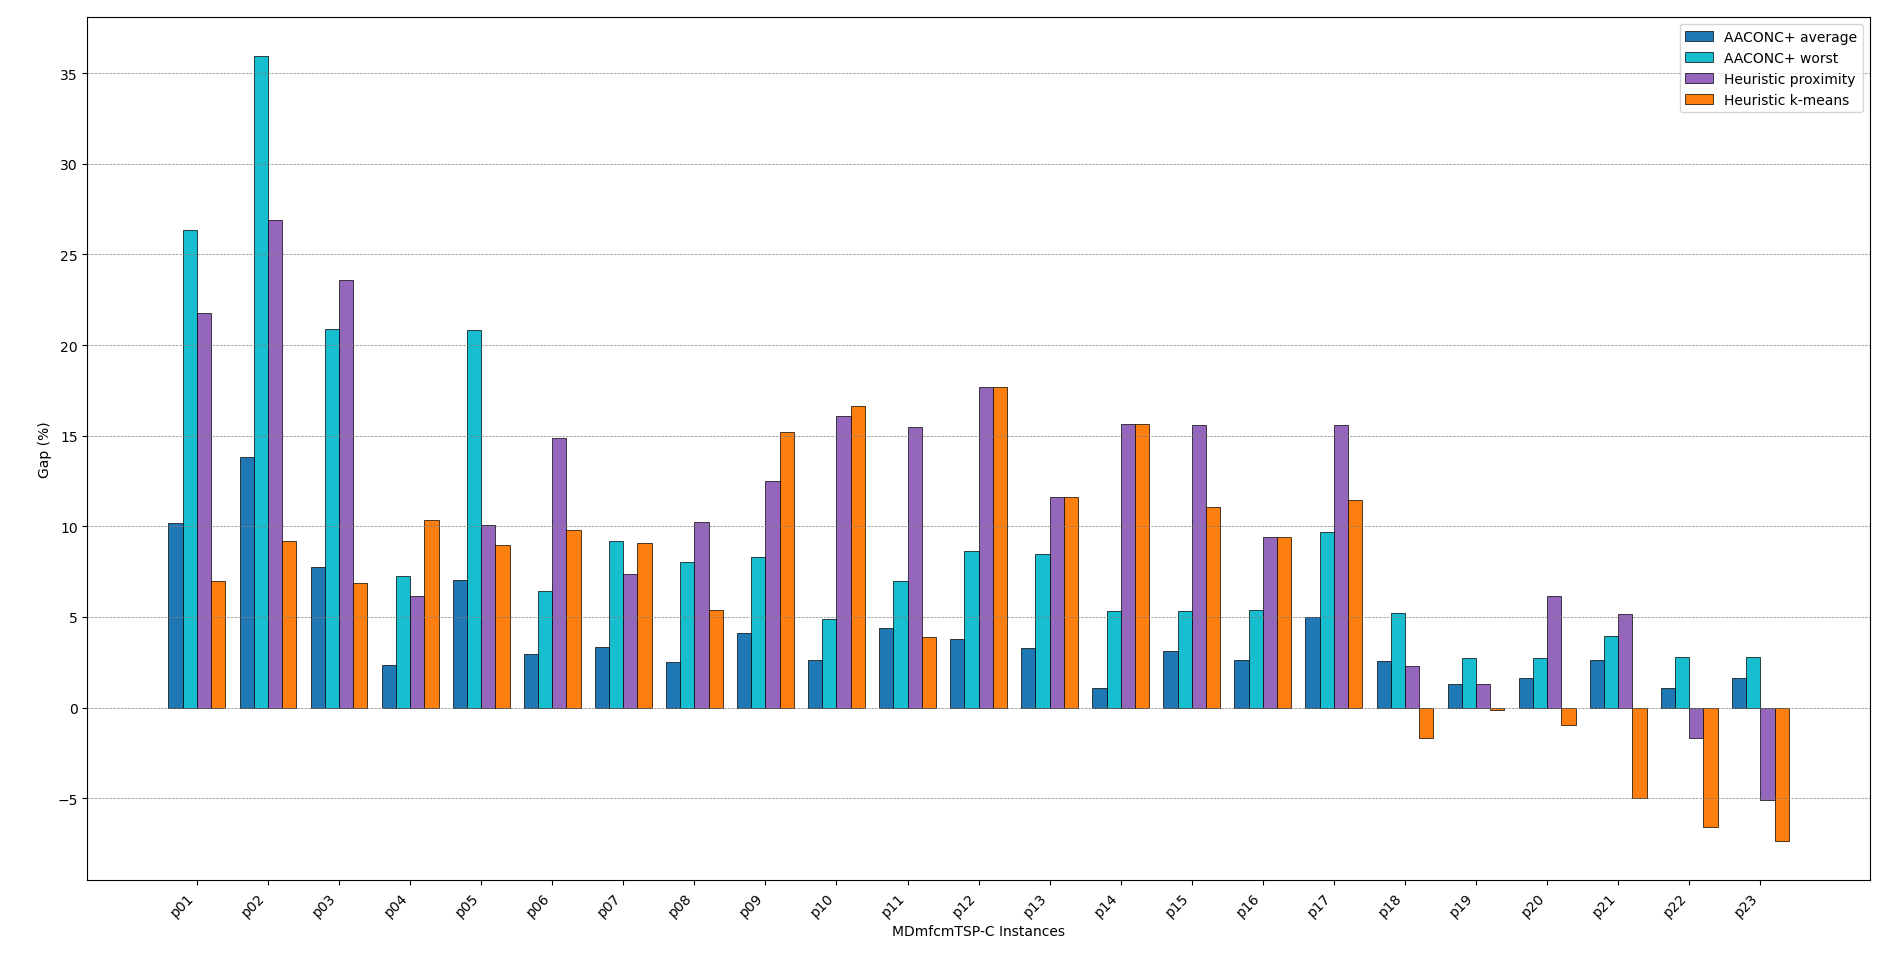
\includegraphics[width=\textwidth]{gaps_to_aco_best}
	\end{figure}
	\begin{figure}[t]
		\caption{Comparison to full local optimization (proximity clustering)}
		\centering
		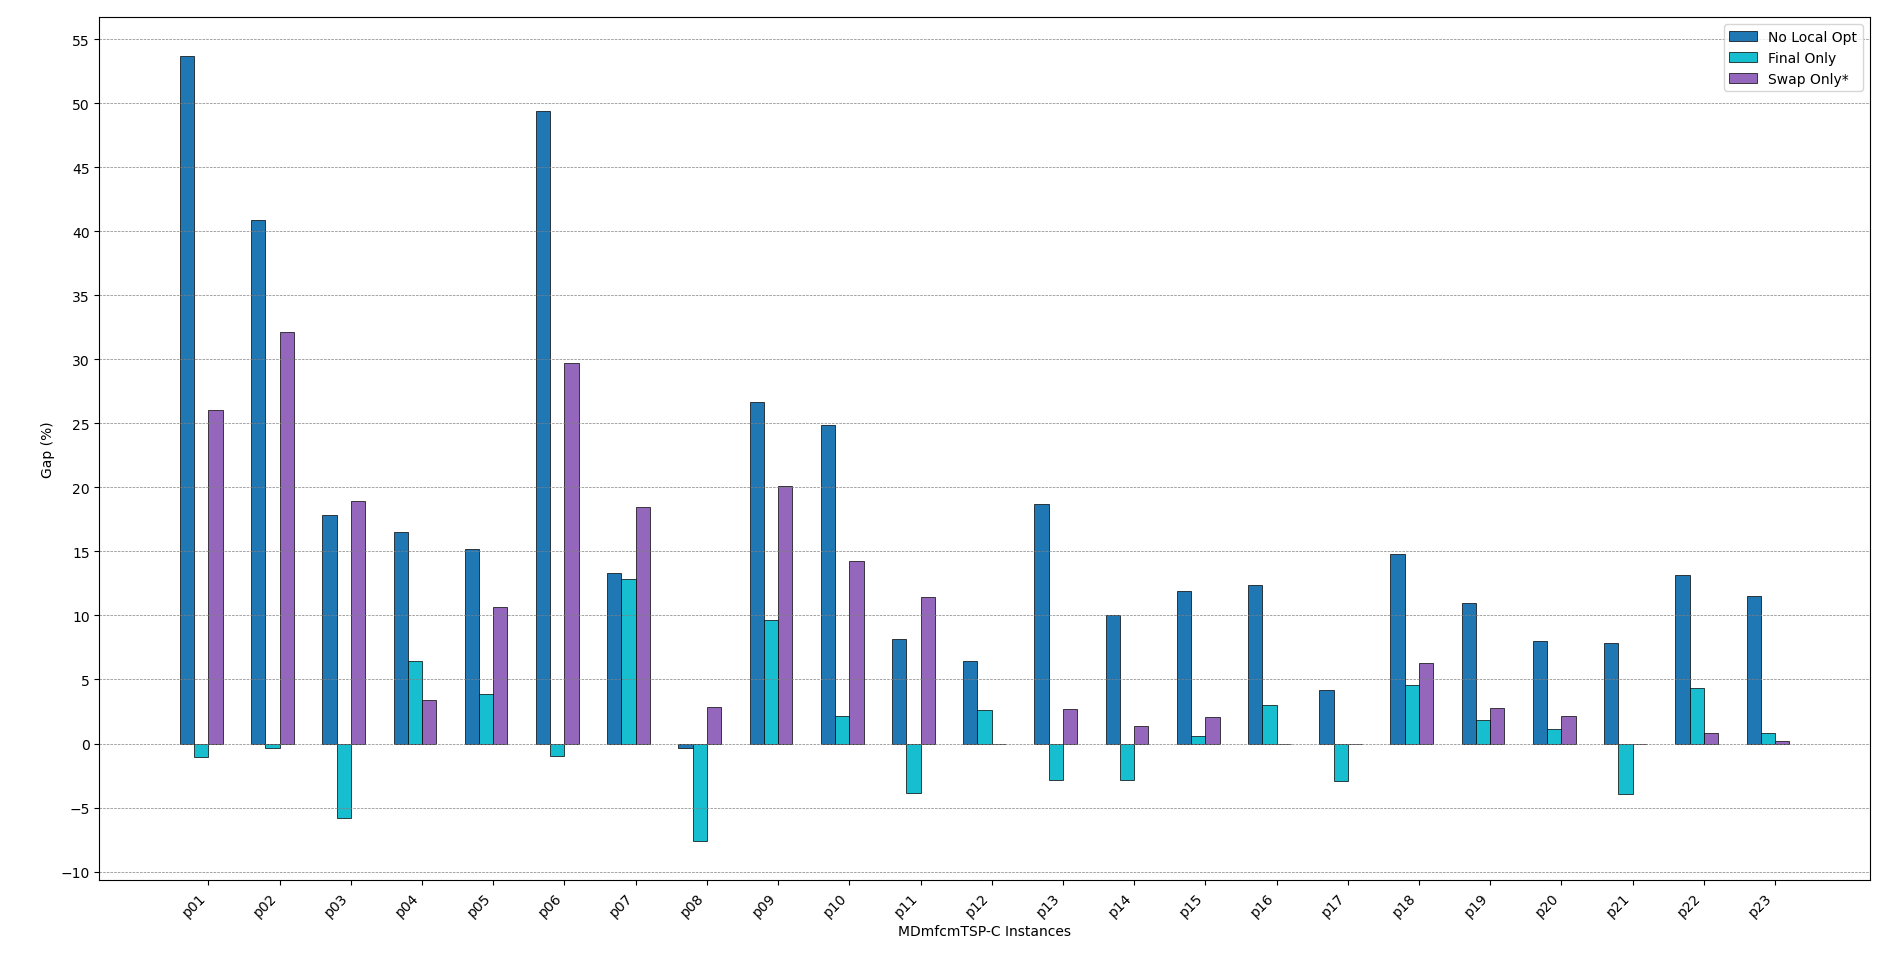
\includegraphics[width=\textwidth]{local_opt_comp_to_full}
	\end{figure}
	\begin{figure}[t]
		\caption{Comparison to full local optimization (k-means clustering)}
		\centering
		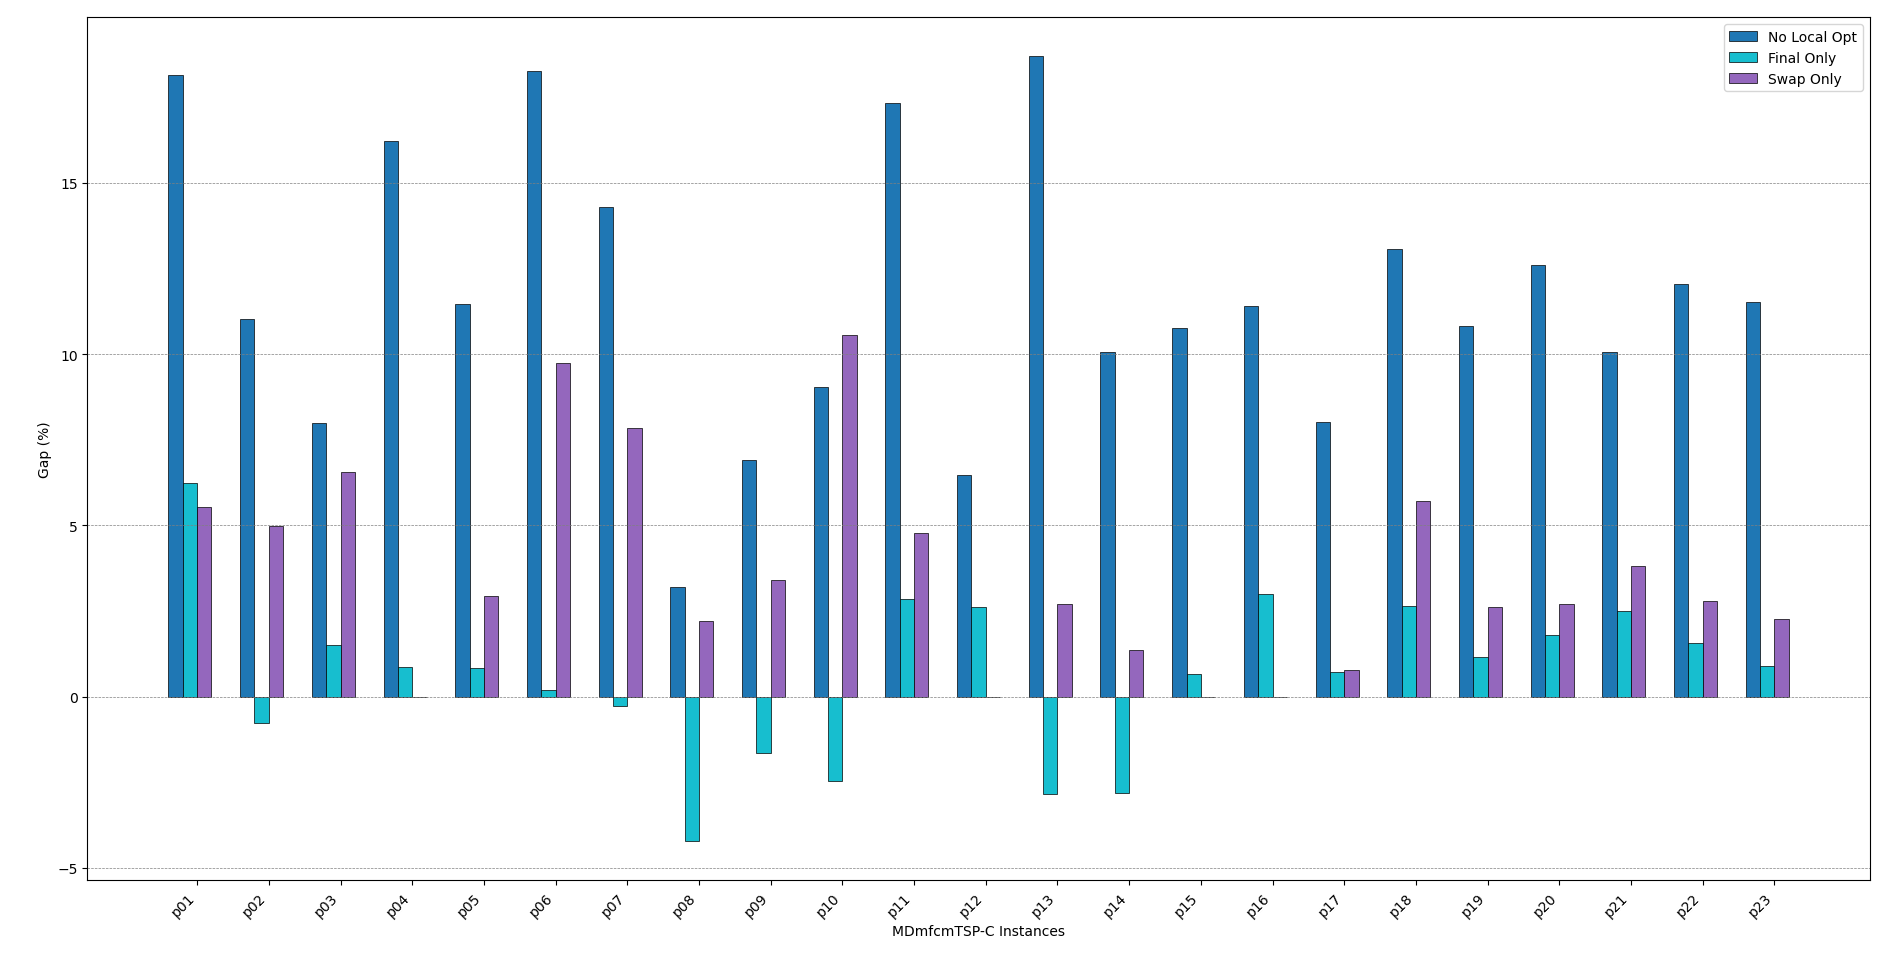
\includegraphics[width=\textwidth]{local_opt_comp_to_full_kmeans}
	\end{figure}
	\begin{figure}[t]
		\caption[width=\textwidth]{kmeans Clustering}
		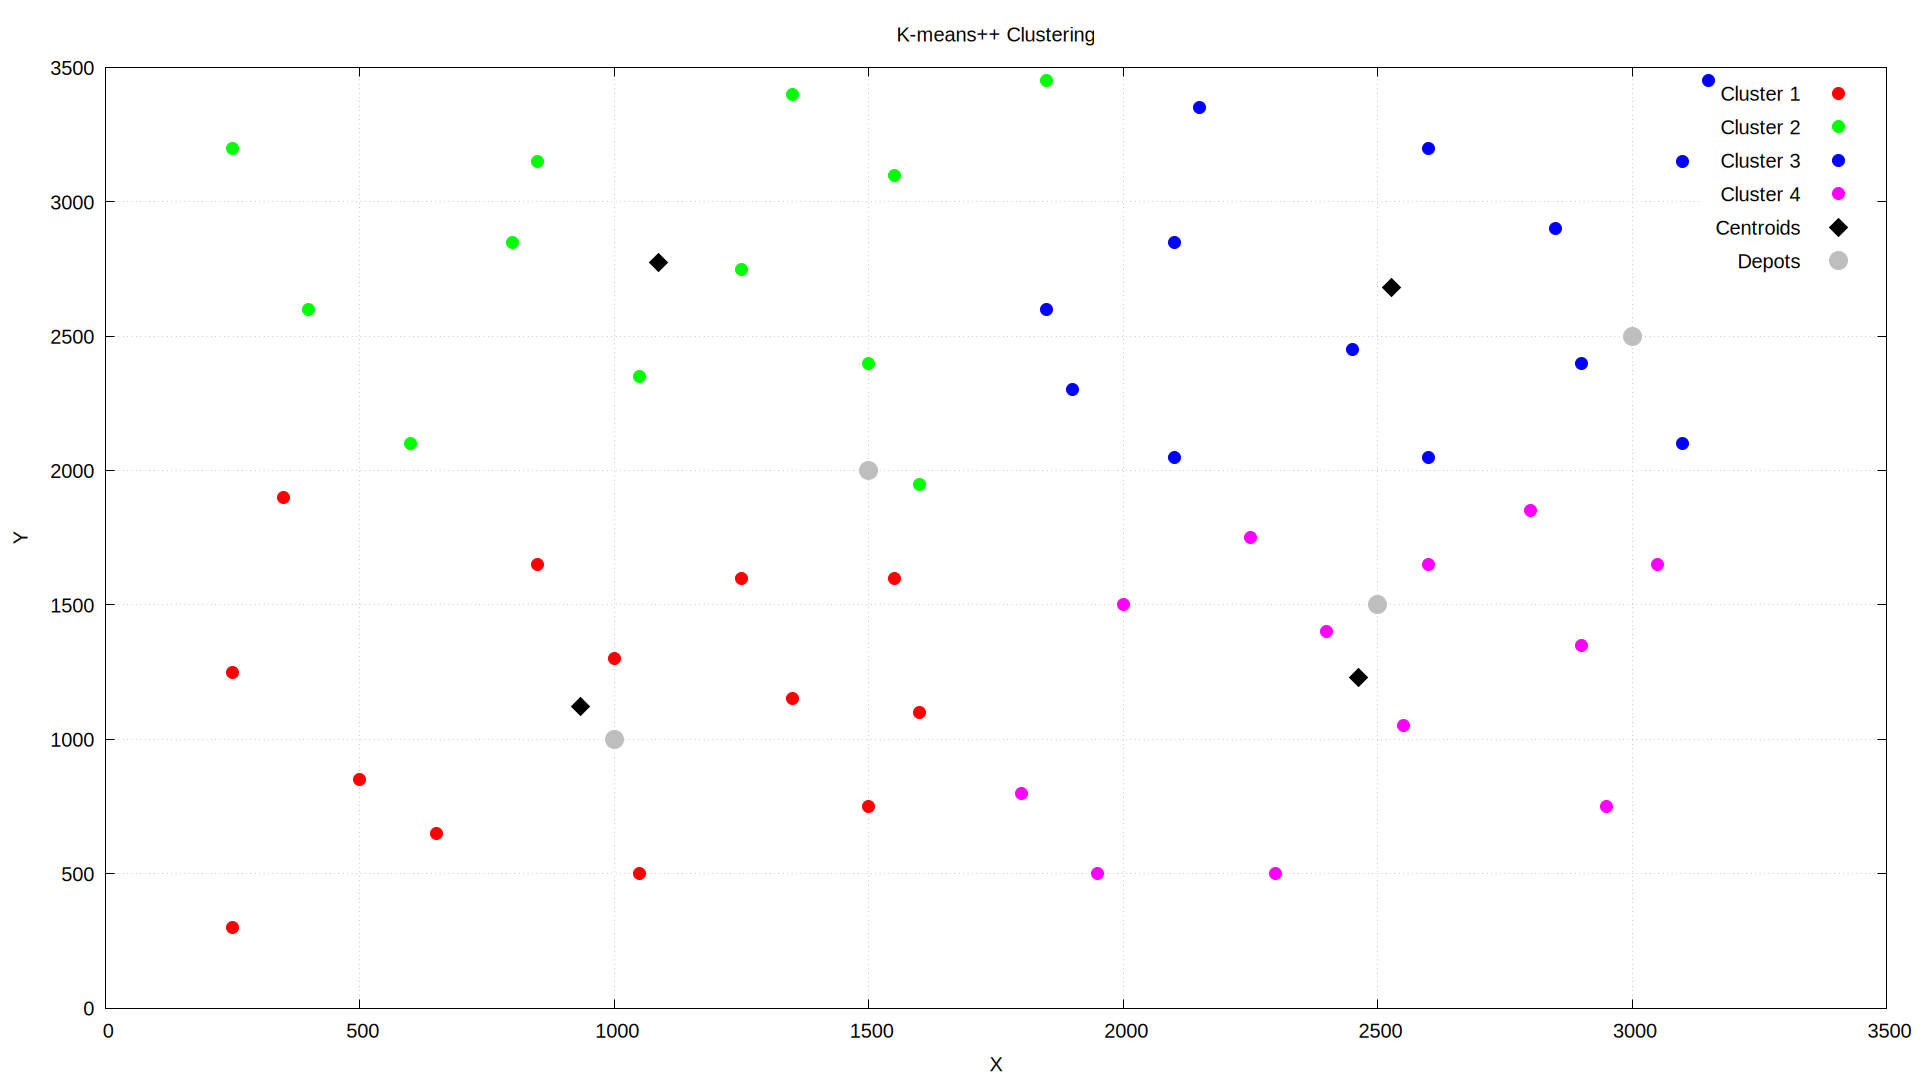
\includegraphics[width=\textwidth]{kmeans-01}
		\centering
	\end{figure}
	

\end{document}